\section{Validating neural network code}
\par{}
A couple of datasets were chosen for validating the developed neural network
code. First is a simple parabola curve data that the network has to approximate
and the second one will be a normalized flight velocity profile data which
the network code has also to approximate. Each problem was explained in detail
as below. \\

\subsection{Parabola problem}
\par{}
The problem framed was to approximate the parabola curve defined with equation
\(y = x^2\) with \(x \in [0,0.5]\).\\

\par{}
A network with three layers and single neuron on each layer, i.e. two hidden
layers and one output layer, was built for this problem. The \(\tanh()\) is
used as the activation function for all the layers and \(mse\) is used as the
loss function for the network. The schematic of network for this problem is
given in \cref{parabola_network_schematic}.\\

\begin{figure}
   \center
    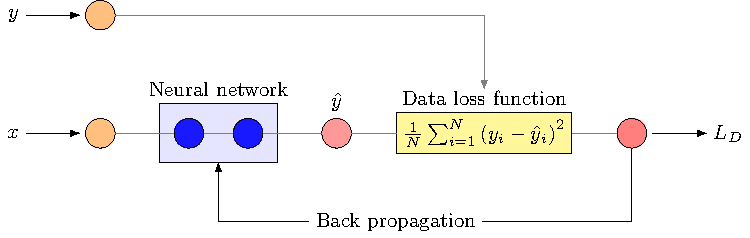
\includegraphics[scale=1]{supportingFiles/01_schematics/02_parabola_network/parabola_network.pdf}
    \caption{Neural network schematic for parabola problem}
    \label{parabola_network_schematic}
\end{figure}

\par{}
Training was performed on the generated data, and the resulting estimated
vs exact profiles were shown in \cref{parabola_result}. It can be seen that the
estimated result is accurate enough to approximate the \(y=x^2\) equation
within the range \(x,y \in [0,0.5]\). Accuracy analysis were not performed as the
motive is to check if the network code works. \\

\begin{figure}
   \center
    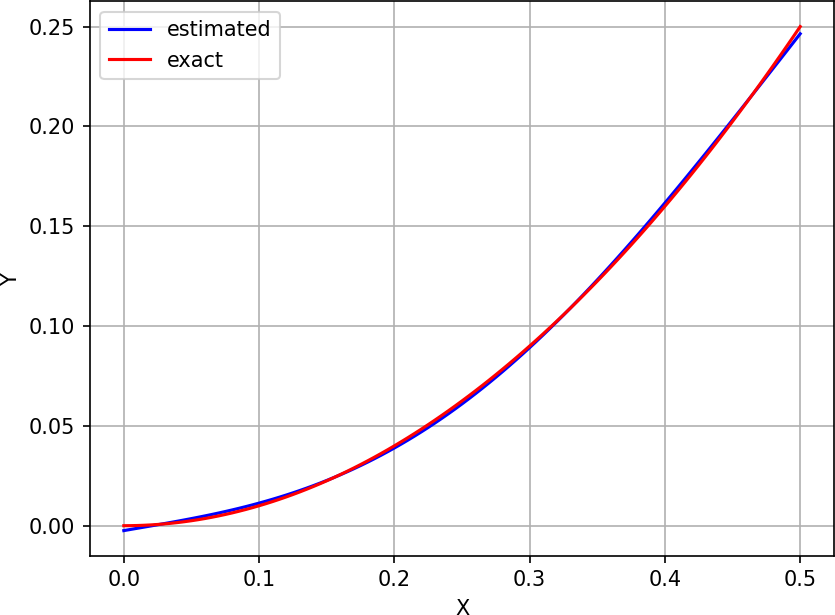
\includegraphics[scale=0.7]{supportingFiles/02_results/01_parabola_datadriven/estimation.png}
    \caption{Estimated vs exact parabola profile by the built neural network}
    \label{parabola_result}
\end{figure}


\subsection{Flight velocity profile}
\par{}
Second validation was performed using a flight velocity profile that was obtained
from the flight dynamics simulation done for an academics assignment work.
The profile was smooth and have both positive and negative curvatures, hence
chosen for the work. \\

\par{}
Schematic of the neural network built for this approximation was shown in
\cref{velocity_profile_network}. The network has 5 neurons with 3 hidden layers
and 1 neuron for the output. Same \(tanh()\) activation function was used
in all the layers. \\

\begin{figure}
   \center
    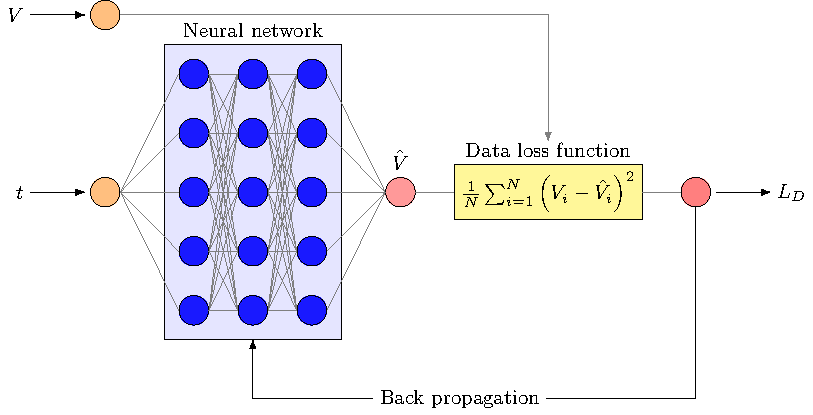
\includegraphics[scale=1]{supportingFiles/01_schematics/03_velocity_profile_network/velocity_profile.pdf}
    \caption{Neural network schematic of flight velocity profile problem}
    \label{velocity_profile_network}
\end{figure}

\par{}
The estimated vs exact flight velocity profiles were given in \cref{velocity_profile_output}.
It can be seen that the estimation matches pretty well with the exact velocity
profile, proving that the network code is correct. Thus, the next step of
enhancing the code to include physics information was performed. \\

\begin{figure}
   \center
    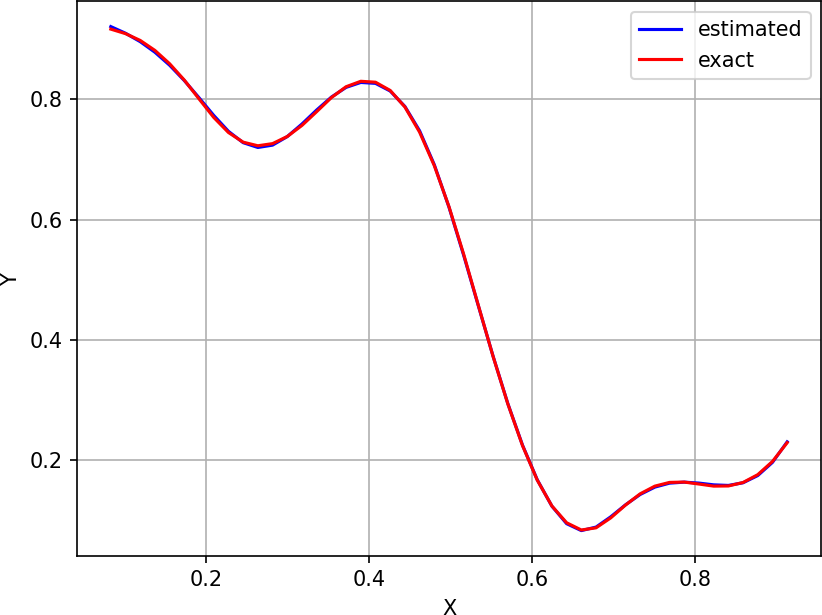
\includegraphics[scale=0.7]{supportingFiles/02_results/02_velocity_profile_dataDriven/estimation.png}
    \caption{Estimated vs exact flight velocity profiles, here X is \(t\) and Y is \(V\)}
    \label{velocity_profile_output}
\end{figure}

